%!TEX TS-program = xelatex
\documentclass[12pt, a4paper]{article}  

\usepackage{etex} % расширение классического tex в частности позволяет подгружать гораздо больше пакетов, чем мы и займёмся далее

%%%%%%%%%% Математика %%%%%%%%%%
\usepackage{amsmath,amsfonts,amssymb,amsthm,mathtools} 
%\mathtoolsset{showonlyrefs=true}  % Показывать номера только у тех формул, на которые есть \eqref{} в тексте.
%\usepackage{leqno} % Нумерация формул слева


%%%%%%%%%%%%%%%%%%%%%%%% Шрифты %%%%%%%%%%%%%%%%%%%%%%%%%%%%%%%%%
\usepackage{fontspec}         % пакет для подгрузки шрифтов
\setmainfont{Linux Libertine O}   % задаёт основной шрифт документа

\defaultfontfeatures{Mapping=tex-text}

% why do we need \newfontfamily:
% http://tex.stackexchange.com/questions/91507/
\newfontfamily{\cyrillicfonttt}{Linux Libertine O}
\newfontfamily{\cyrillicfont}{Linux Libertine O}
\newfontfamily{\cyrillicfontsf}{Linux Libertine O}

\usepackage{unicode-math}     % пакет для установки математического шрифта
\setmathfont{Asana Math}      % шрифт для математики

\usepackage{polyglossia}      % Пакет, который позволяет подгружать русские буквы
\setdefaultlanguage{russian}  % Основной язык документа
\setotherlanguage{english}    % Второстепенный язык документа


%%%%%%%%%% Работа с картинками %%%%%%%%%
\usepackage{graphicx}                  % Для вставки рисунков
\usepackage{graphics} 
\graphicspath{{images/}{pictures/}}    % можно указать папки с картинками
\usepackage{wrapfig}                   % Обтекание рисунков и таблиц текстом
\usepackage{subfigure}                 % для создания нескольких рисунков внутри одного


%%%%%%%%%% Работа с таблицами %%%%%%%%%%
\usepackage{tabularx}            % новые типы колонок
\usepackage{tabulary}            % и ещё новые типы колонок
\usepackage{array}               % Дополнительная работа с таблицами
\usepackage{longtable}           % Длинные таблицы
\usepackage{multirow}            % Слияние строк в таблице
\usepackage{float}               % возможность позиционировать объекты в нужном месте 
\usepackage{booktabs}            % таблицы как в книгах!  
\renewcommand{\arraystretch}{1.3} % больше расстояние между строками





% Заголовок
\author{Перевышин Юрий} 
\title{Домашнее задание 2}
\date{\today}

\begin{document} 

\maketitle

\section{Поп-арт}




\begin{figure}[H]
	\begin{minipage}[h]{0.32\linewidth}
		\center{
\includegraphics[width=1\linewidth, height=6cm]{pop3.pdf}} \\
	\end{minipage}
	\hfill
	\begin{minipage}[h]{0.32\linewidth}
		\center{\includegraphics[width=1\linewidth, height=6cm]{pop5.pdf}} \\
	\end{minipage}
\hfill
\begin{minipage}[h]{0.32\linewidth}
	\center{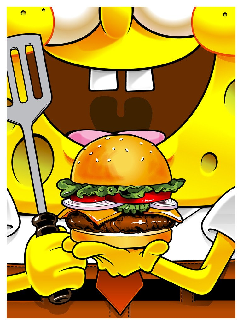
\includegraphics[width=1\linewidth, height=6cm]{pop8.pdf}} \\
\end{minipage}

	\vfill
	\begin{minipage}[h]{0.32\linewidth}
	\center{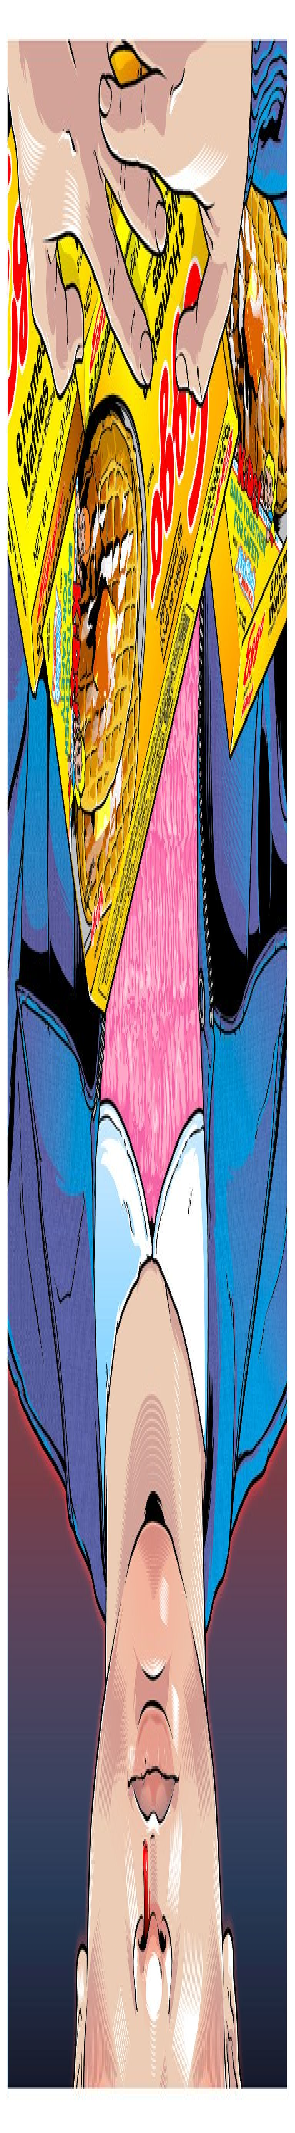
\includegraphics[width=1\linewidth, height=6cm, angle=180]{pop2.pdf}} \\
\end{minipage}
\hfill
\begin{minipage}[h]{0.32\linewidth}
	\center{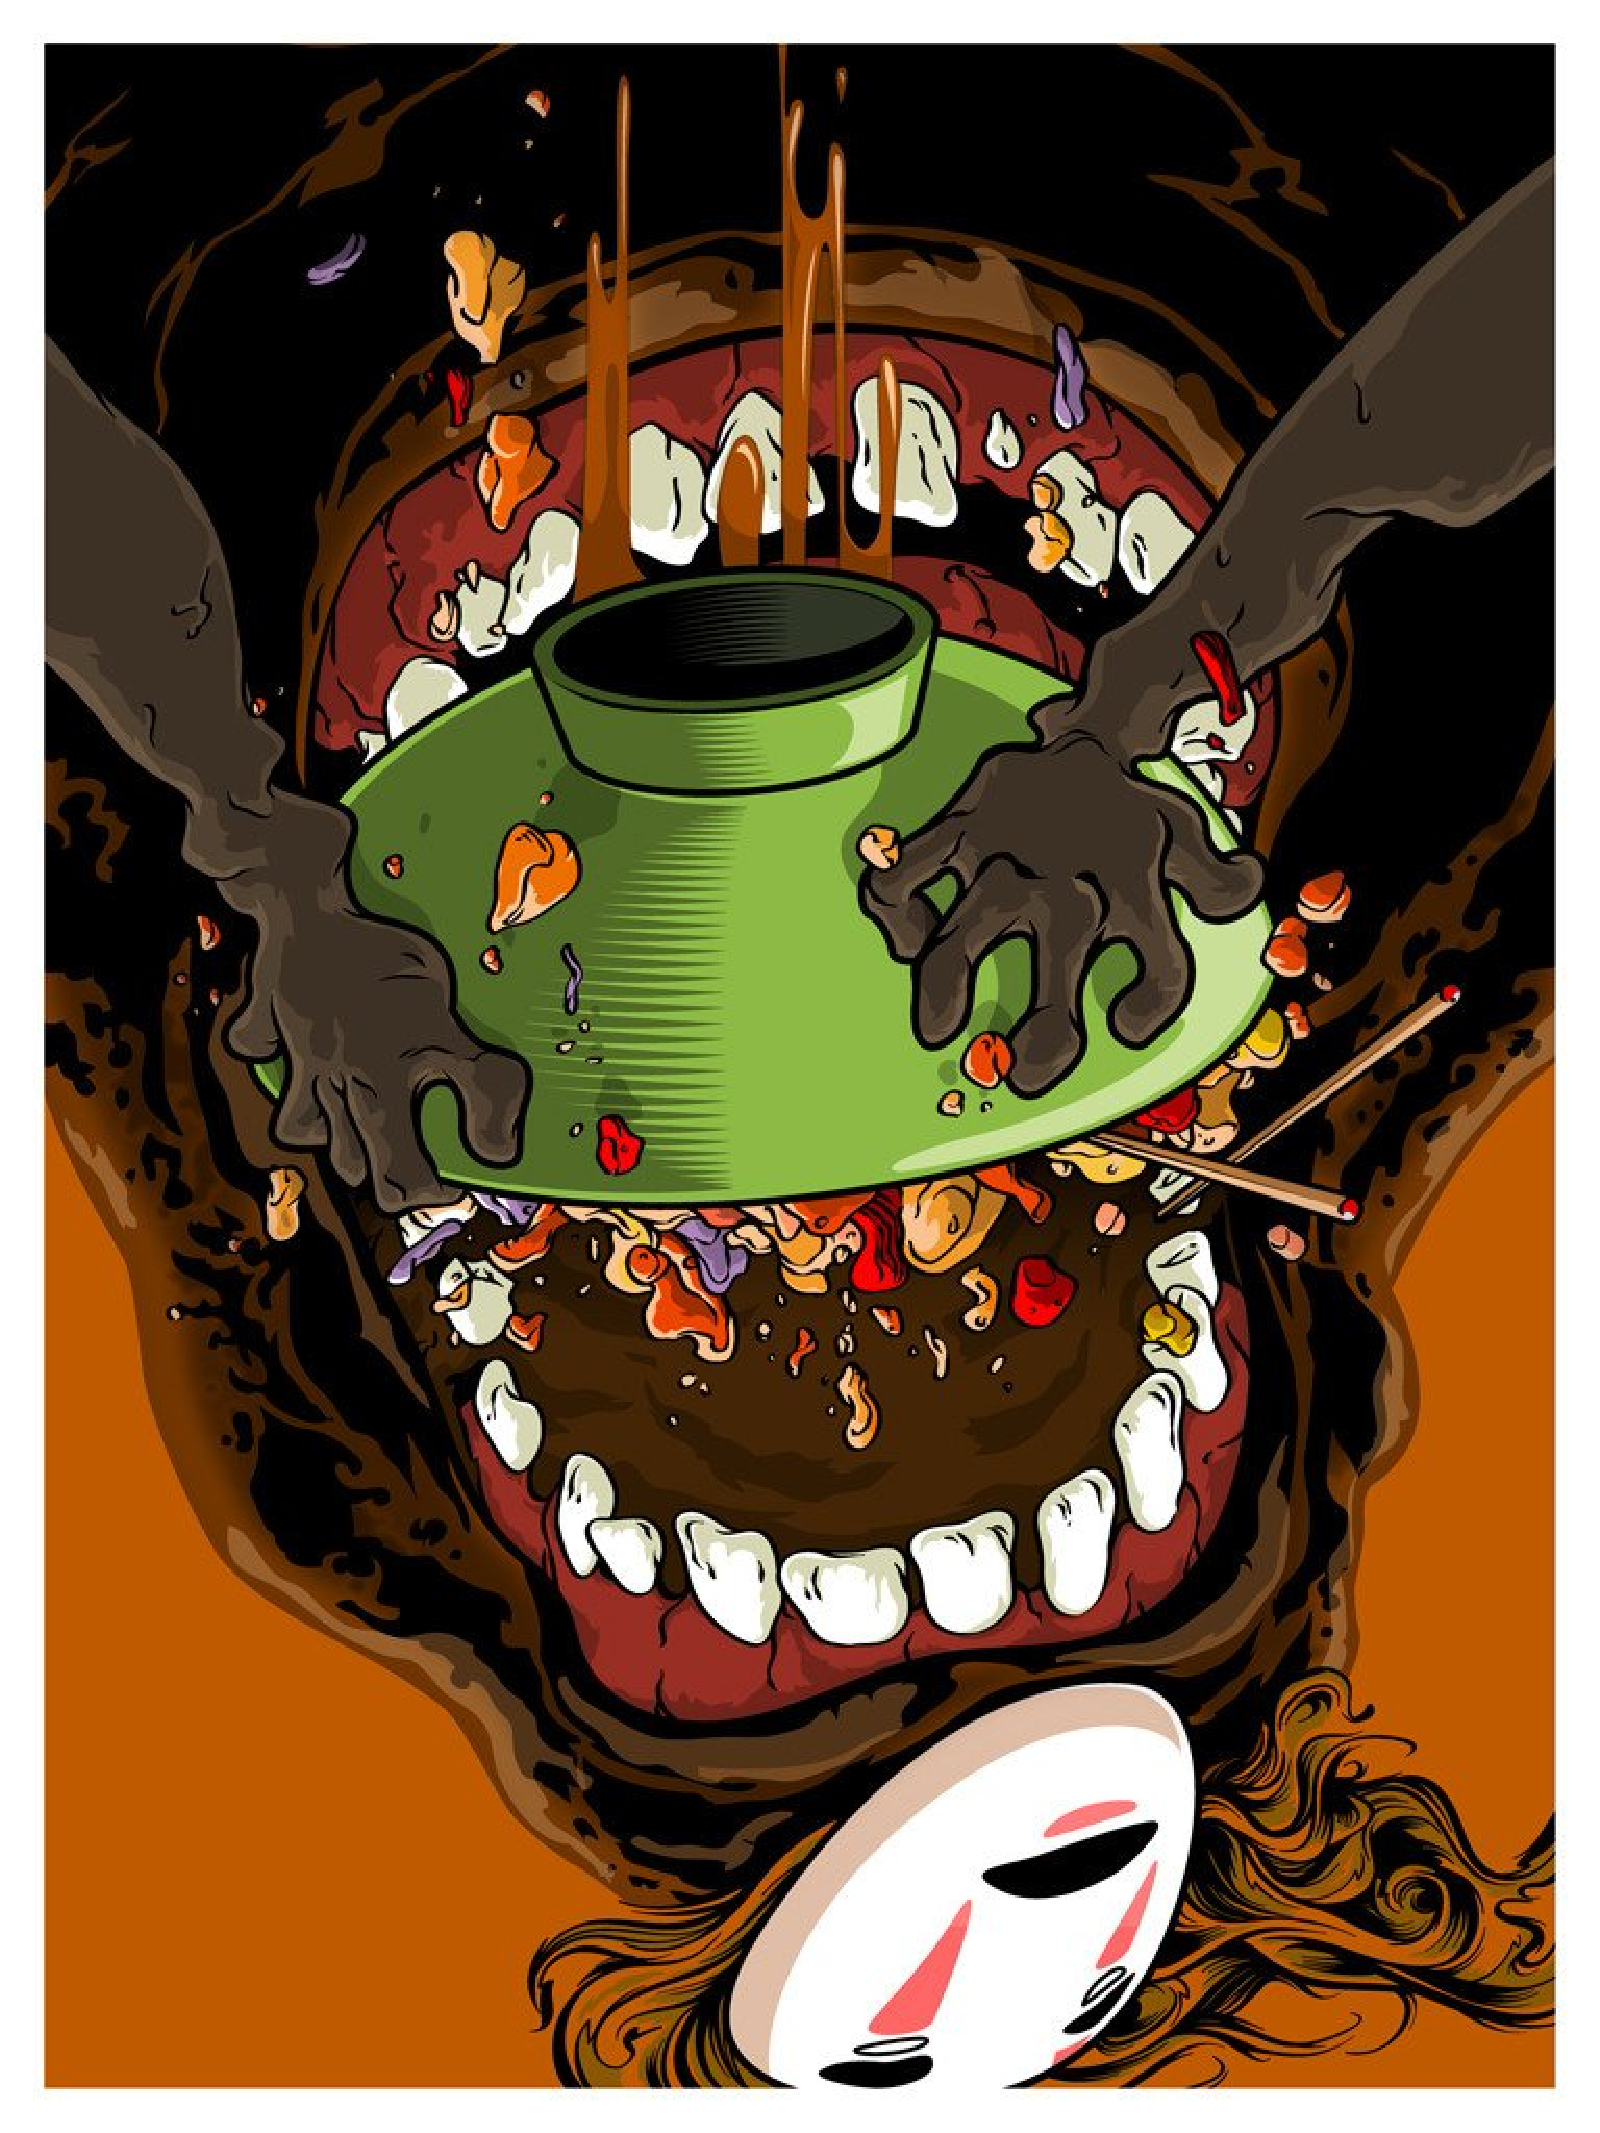
\includegraphics[width=1\linewidth,height=6cm, angle=180]{pop6.pdf}} \\
\end{minipage}
\hfill
\begin{minipage}[h]{0.32\linewidth}
	\center{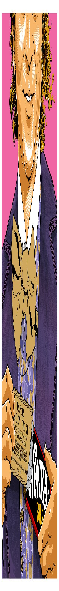
\includegraphics[width=1\linewidth, height=6cm]{pop7.pdf}} \\
\end{minipage}

\end{figure}



\end{document}